\documentclass[14pt]{extarticle}

\DeclareMathSizes{14}{14}{15}{12}

\renewcommand{\normalsize}{\fontsize{14}{16}\selectfont}


% Language setting
% Replace `english' with e.g. `spanish' to change the document language
\usepackage[english]{babel}
\usepackage{graphicx}
\graphicspath{ {./images/} }
% Set page size and margins
% Replace `letterpaper' with `a4paper' for UK/EU standard size

\usepackage[letterpaper,top=2cm,bottom=2cm,left=3cm,right=3cm,marginparwidth=1.75cm]{geometry}

% Useful packages
\usepackage{amsmath}
\usepackage{graphicx}
\usepackage[colorlinks=true, allcolors=blue]{hyperref}

\title{TP2 Automatique}

\begin{document}
\maketitle


\section{}

Soit $e(t)$ une impulsion de Dirac, $s(t)$ la réponse impulsionnelle du bloqueur d'ordre 0 et $u(t)$ le signal echelon unite. 


\[ s(t) = u(t) - u(t-T_e) \xrightarrow{\text{TL}} S(p) = \frac{1}{p} - \frac{e^{-pT_e}}{p} = \frac{1-e^{pT_e}}{p}\]
\[E(P) = 1\] 
\[B_0(P) = \frac{S(p)}{E(p)} = \frac{1-e^{pT_e}}{p}\] 


\section{}
\[A(z) = TZ[\frac{G_0(p)}{p}]\]
Dans le domaine temporel, on a :
\[TL^{-1}[\frac{G_0(p)}{p}] = TL^{-1}[\frac{1+p}{p^3}] = TL^{-1}[\frac{1}{p^2}] + TL^{-1}[\frac{1}{p^3}] = \frac{t^2}{2}u(t) + tu(t)\]

\[A(z) = TZ[\frac{t^2}{2}u(t) + tu(t)] = \frac{z(z+1)T_{e}^2}{2(z-1)^3} + \frac{zT_e}{(z-1)^2} = \frac{z(z+1)T_e^2+2z(z-1)T_e}{2(z-1)^3}\] 
\[G(z)= (1-z^{-1})A(z) = \frac{T_e(z(2+T_e)+T_e -2)}{2(z-1)^2}\]

\section{}

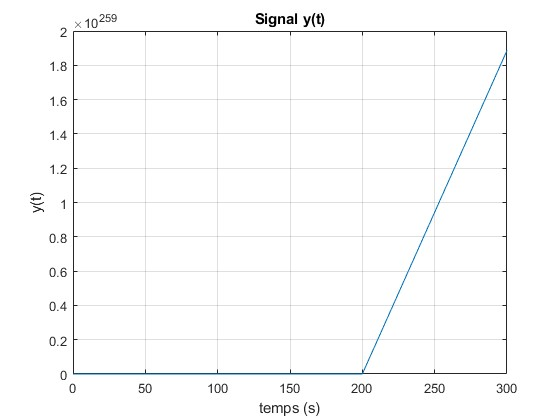
\includegraphics{untitled.jpg}

\section{}
\[H(z) = \frac{C(z)G(z)}{1+C(z)G(z)} = \frac{KT_e(z(2+T_e) + T_e - 2)}{2(z-1)^2 + KT_e(z(2+T_e)+T_e - 2)}\] 

Soit D(z) le polynome caracteristique au dénominateur de H(z) :
\[D(z) = 0 \Leftrightarrow 2(z-1)^2 + KT_e(z(2+T_e)+T_e - 2) = 0 \]

\[\Leftrightarrow 2z^2 + z(KT_e(2+T_e) - 4) + KT_e(T_e - 2) +2 = 0 \]

\[\Delta = [(KT_e(2 + T_e)-4)]^2 - 8[KT_e(T_e -2) +2] = KT_e^2[K(2+T_e)^2 - 16] \]

pour $\Delta = 0$ on a : 
\[K_0 = 0 \text{ et } K = \frac{16}{(2+T_e)^2}\]
\section{}
Le systeme est stable si les poles de la fonction de transfert $H(z)$ autrement dit les racines de $D(z)$ ont un module strictement inferieur a 1.
\break
Les modules des 2 racines sont compris entre 0 et 1 pour $0<K<20$.
\section{}
Les conditions de stabilite d'apres le critere de Jury sont :
\begin{itemize}
    \item $D(1) = 2KT_e^2 > 0 \Leftrightarrow K > 0$
    \item $D(-1) = 8-4KT_e>0 \Leftrightarrow K<2/T_e = 2/0.1 = 20$
\end{itemize}
D'ou $0<K<20$.

\section{}
G(z) contient deux integrateurs dans son expression, on peut donc en deduire les resultats suivants :
\begin{itemize}
    \item \[\epsilon_p = \lim_{z\to1} \frac{1}{1+KG(z)} = 0\]
    \item \[\epsilon_v = \lim_{z\to1} \frac{z-1}{z} \times \frac{1}{1+KG(z)} = 0\]
\end{itemize}
Le systeme est donc precis pour tout K.

\section{}
\[{S(Z)} = H(Z)E(Z) \]
\[\Leftrightarrow S(z) = \frac{z^{-1}KT_e(2+T_e) + z^{-2}KT_e(T_e-2) }{2+z^{-1}[(KT_e(2+T_e) - 4)] + z^{-2} [KT_e(T_e-2) +2]} E(Z)\]
\[\Leftrightarrow (2+z^{-1}[(KT_e(2+T_e) - 4)] + z^{-2} [KT_e(T_e-2) +2])S(z)\]  \[= (z^{-1}KT_e(2+T_e) + z^{-2}KT_e(T_e-2))E(z)\] 
\[\Leftrightarrow s_k = \frac{1}{2} [KT_e(2+T_e)e_{k-1} + KT_e(T_e - 2)e_{k-2} - ((KT_e(2+T_e)-4))s_{k-1} \] \[ - (KT_e(T_e-2)+2)s_{k-2}]\]
\end{document}
	
